\documentclass[10pt]{article}
\textheight=9.25in \textwidth=7in \topmargin=-.75in
 \oddsidemargin=-0.25in
\evensidemargin=-0.25in
\usepackage{url}  % The bib file uses this
\usepackage{graphicx} %to import pictures
\usepackage{amsmath, amssymb}
\usepackage{theorem, multicol, color}
\usepackage{gfsartemisia-euler}

\setlength{\intextsep}{5mm} \setlength{\textfloatsep}{5mm}
\setlength{\floatsep}{5mm}
\setlength{\parindent}{0em} % new paragraphs are not indented
\setcounter{MaxMatrixCols}{20}
\usepackage{caption}
\captionsetup[figure]{font=small}


%%%%  SHORTCUT COMMANDS  %%%%
\newcommand{\ds}{\displaystyle}
\newcommand{\Z}{\mathbb{Z}}
\newcommand{\arc}{\rightarrow}
\newcommand{\R}{\mathbb{R}}
\newcommand{\N}{\mathbb{N}}
\newcommand{\Q}{\mathbb{Q}}
\renewcommand{\P}{\mathbb{P}}
\newcommand{\blank}{\underline{\hspace{0.33in}}}
\newcommand{\qand}{\quad and \quad}
\renewcommand{\stirling}[2]{\genfrac{\{}{\}}{0pt}{}{#1}{#2}}
\newcommand{\dydx}{\ds \frac{d y}{d x}}
\newcommand{\ddx}{\ds \frac{d}{d x}}
\newcommand{\dvdx}{\ds \frac{d v}{d x}} 
\newcommand{\solution}{\color{blue} Solution: \color{black}}
%%%%  footnote style %%%%

\renewcommand{\thefootnote}{\fnsymbol{footnote}}

\pagestyle{empty}

\begin{document}

\begin{flushright}
Chandler Justice - A02313187
\end{flushright}
\noindent \underline{\hspace{3in}}\\
\textbf{MATH 6400:} Quiz \#3\\
\textbf{Due:} January 28, 2026 @ 23:59\\


	\begin{enumerate}
		\item Assume the figure below is a regular pentagon with each side being length $1$.  Prove that $x$ is the \emph{Golden Ratio}; that is $x = \frac{1+\sqrt{5}}{2}$.  \textsf{Hint:} Find similar triangles and parallel lines to show that $x$ satisfies $$\frac{x}{1} = \frac{1}{x-1},$$
		
		
		\begin{center}
			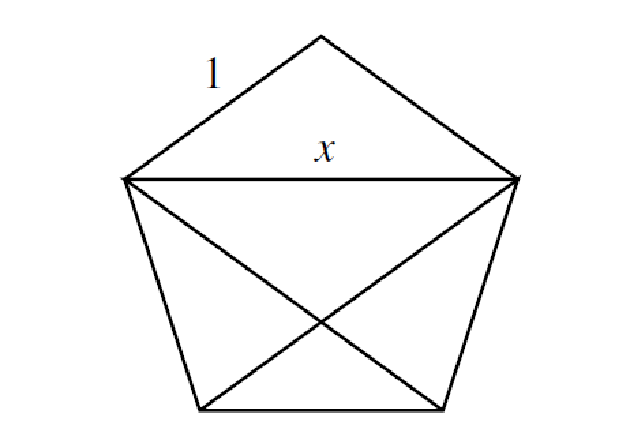
\includegraphics[scale=0.5]{Pentagon_with_unit_side_and_x_diag.pdf}
		\end{center}

        \solution We can see since all sides of the pentagon have length $1$, this means any line between two non-adjacent corners will have the same length, $x$. We can then label the points as outlined in the figure below

        \begin{center}
            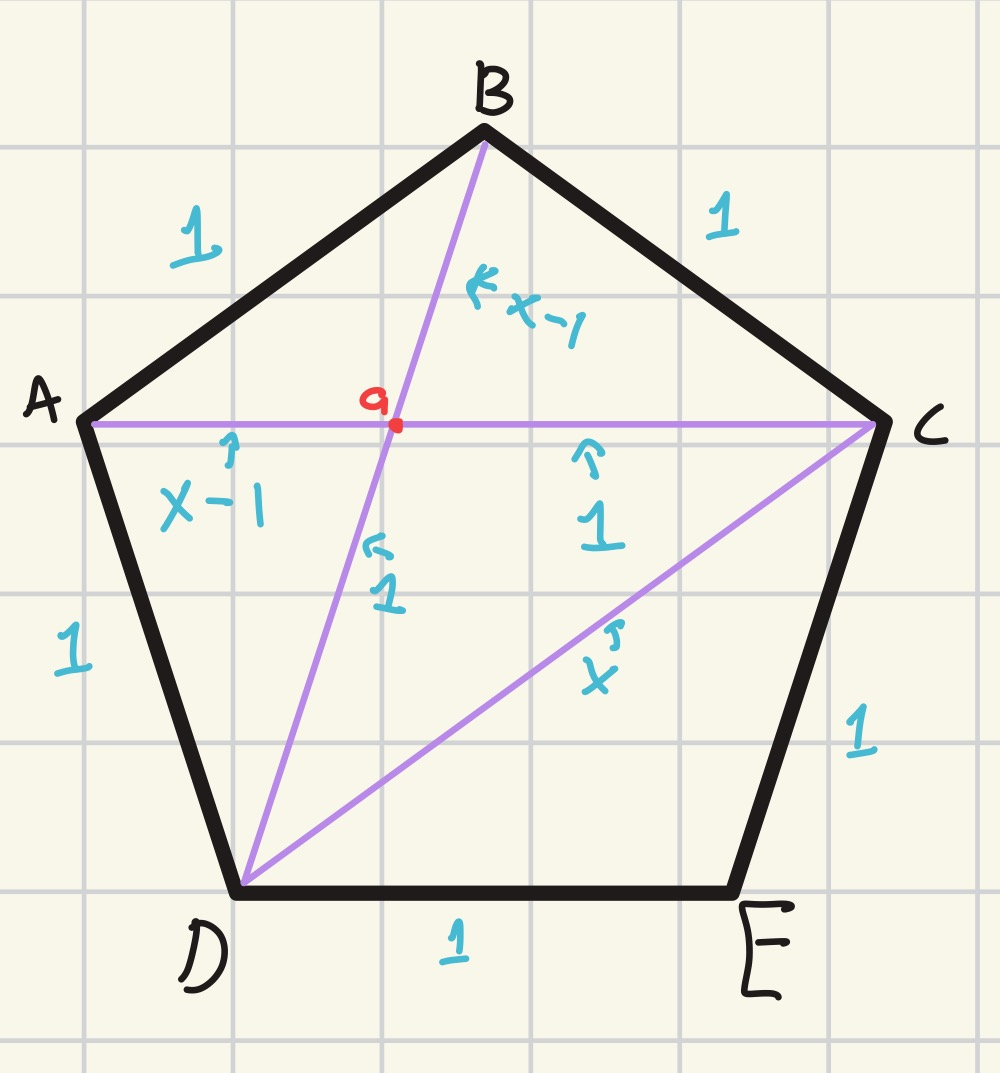
\includegraphics[scale=0.2]{fig1.jpeg}
        \end{center}

        From here, we can construct diagonals $AC$ and $BD$, and denote the intersection of these lines $a$. By transferring the line $DE$ to the line created by $aC$ as described in Euclid I.2, we can see the length of $aC$ is $1$. We can then construct the line $CD$, which as mentioned earlier will have length $x$.\\

        It becomes apparent $aAB$ forms a triangle similar to $aCD$, as both form isosceles triangles which are corresponding in their ratios of lengths. We can see $\frac{AB}{aB} = \frac{CD}{aC} \Rightarrow \frac{1}{x-1} = \frac{x}{1}$. Using algebraic manipulation, we can then solve for x:
        \begin{align*}
            \frac{x}{1} &= \frac{1}{x-1}\\
            (x - 1)\frac{x}{1} &= (x - 1)\frac{1}{x-1}\\
            x(x-1) &= 1\\
            x^2 - x - 1 &= 0\\
            -x^2 + x + 1 &= 0\\
            x &= \frac{-(-1)^2 \pm \sqrt{1 - 4(-1)(1)}}{2(-1)} && \text{(by \textit{the} quadratic formula)}\\
            x &= \frac{1 + \sqrt{5}}{2} = \varphi
            \end{align*}
		$\hfill\blacksquare$
		\item Given the result of the first prompt, describe how to construct a regular pentagon using only straightedge and compass. You may assume that $\varphi$ has been constructed (that is, some length has been constructed that measures $\varphi$), and that `numbers' (distances or lengths of line segments) can be transferred. 
		
		\textsf{Suggestion:} Start by assuming I have the bottom side of the pentagon laid down and that its length is $1$.  Then use the Golden Ratio (which you may assume has been constructed and is transferable). 
		
        \solution Start with the bottom of the pentagon laid down with length $1$ and denote its endpoints $A$ and $B$. Using the compass, construct a circle of radius $\varphi$ centered at $B$; repeat this construction centered at $A$. Call the circles centered at $A$ and $B$ $c_1$ and $c_2$, respectively. Denote the point of intersection of these circles $C$. Construct a circle centered at $C$ with radius $1$ denoted $c_3$. Then, find the intersection of $c_3$ and $c_1$, denote this intersection $F$, repeat for $c_2$ and $c_3$ denoting this intersection $E$. Construct the lines $AB, AE, EC, CF$ and $FB$, which create a pentagon.

        \begin{center}
            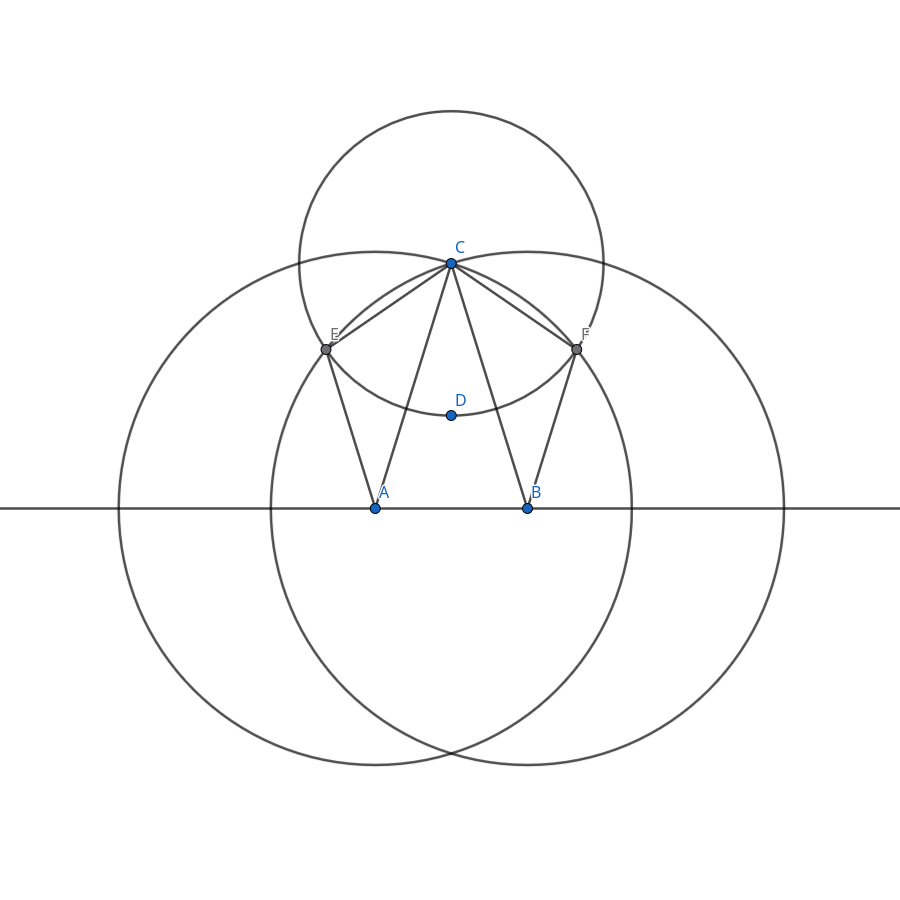
\includegraphics[scale=0.2]{fig4.png}
        \end{center}

		\item Trisect a right angle using straightedge and compass.  A bullet-proof Euclid-style proof is not necessary, but the construction should be explained enough to be convincing.

            \solution Below is a construction I performed using Geogebra's \textit{Geometric Constructions} tool, which allows for a digital equivalent of a straight edge and compass. 
            \begin{center}
                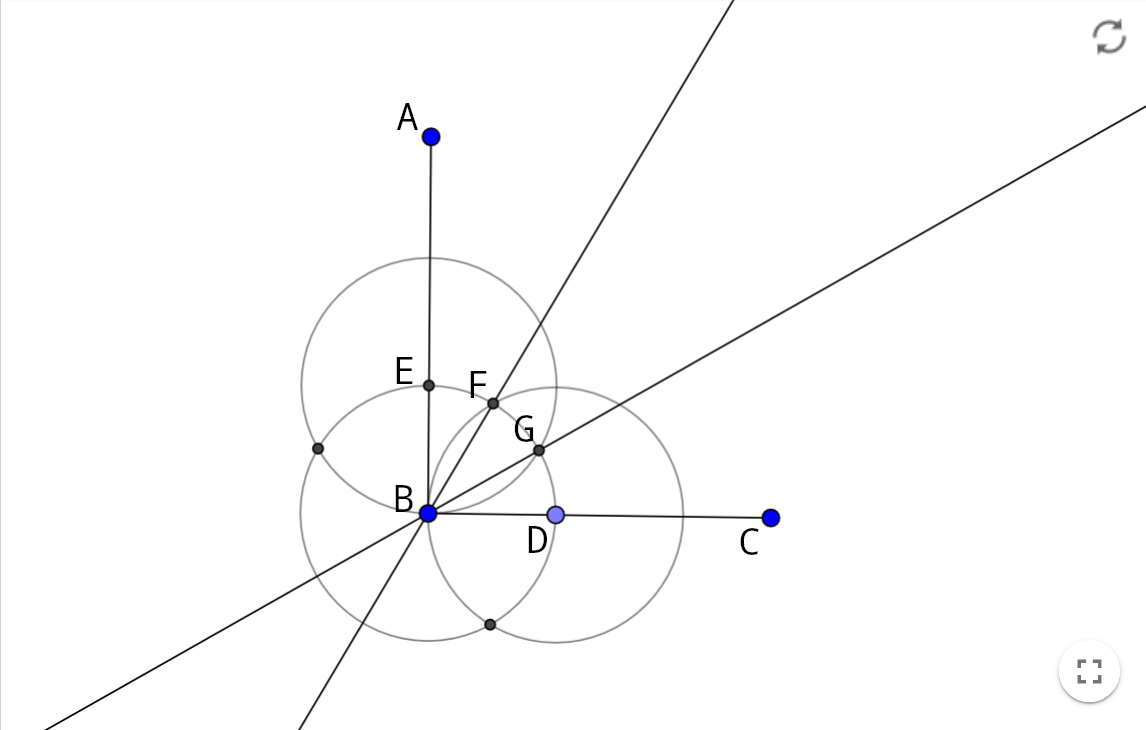
\includegraphics[scale=0.3]{fig2.png}
            \end{center}

            First I constructed the right angle by creating two tangent lines\footnote{I am assuming the right angle is given, so I used the angle tool to adjust the lines until the lines were tangent}. From there, mark point $D$, which will be our unit length, on line $BC$ and create a circle which centers around point $B$, denote the intersection with the line $AB$ as point $E$. Create another circle with radius of line $BE$ centered at point $E$. Note the intersection of these circles in the right angle as point $G$. The points $BEG$ form an equilateral triangle, meaning all interior angles of the triangle are 60 degrees. Recall the interior angle of a right triangle is 90 degrees. Since the triangle $BEG$ shares the line $BE$ with the right angle, we can see $\frac{BE}{BG} = \frac{2}{3}\frac{BE}{BD}$. If we mirror this construction by creating another circle centered at point $D$ and then noting the intersection between this circle and our original circle as point $F$, then we can see we get an identical result where $\frac{BD}{BF} = \frac{2}{3} \frac{BD}{BE}$. Therefore, we can see $\frac{BE}{BF} = \frac{BF}{BG} = \frac{BG}{BD} = \frac{1}{3} \frac{BE}{BD}$, meaning the lines $BF$ and $BG$ trisect the angle created by lines $BD$ and $BE$.



		\item Trisect a line segment.  \textsf{For 6400 people}:  Provide a bullet-proof Euclid-style proof.

            \solution Once again using Geogebra's \textit{Geometric Constructions} tool, I created this figure using the straightedge and compass

            \begin{center}
                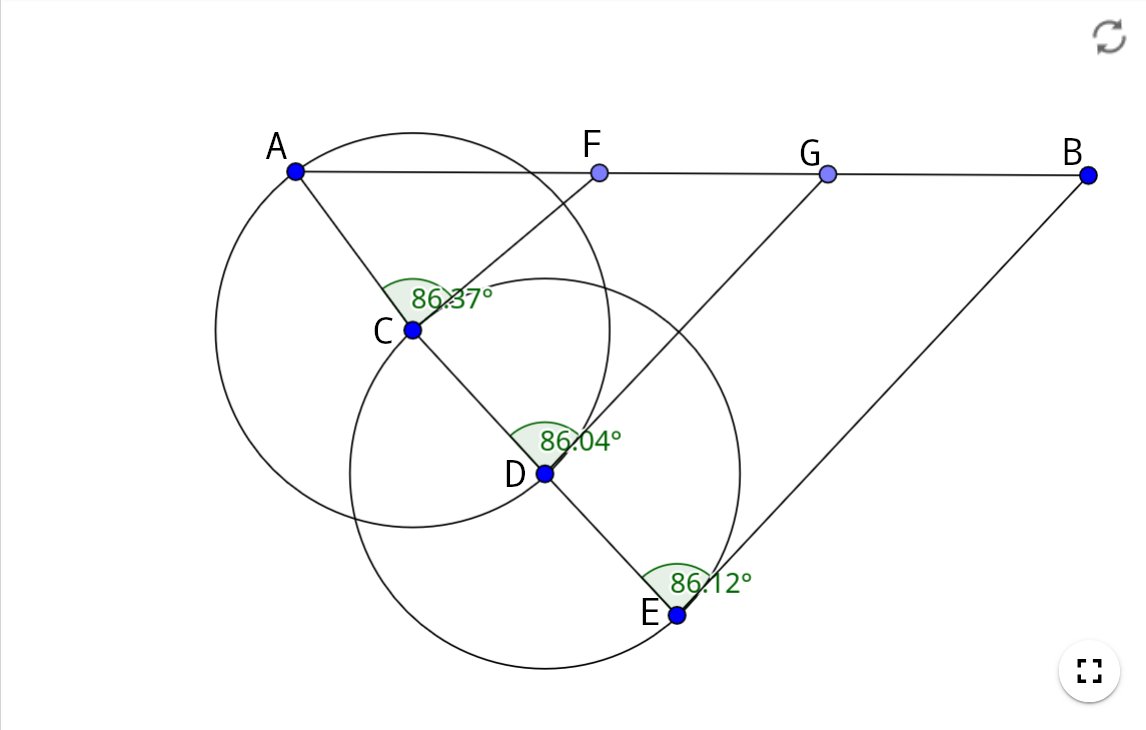
\includegraphics[scale=0.25]{fig3.png}
            \end{center}
		    
            We label the endpoints of the line segment $A$ and $B$. From there we draw a line segment out from $A$ and denote the endpoint $C$. From here, using a compass we draw a circle whose radius is the length $AC$. We can then construct $CD$ to be the line segment extending the line $AC$ to the edge of the circle. From there we can draw a circle from $C$ towards the point $D$, and construct the line and point $DE$ and $E$ respectively with the same technique as $CD$. From here, construct the line $BE$.\\

            Using the angle of line $BE$, Construct lines between the points $C$ and $D$ which intersect with the line segment $AB$; we now have the lines $CF$ and $DG$. We can then see we have triangles $ABE, ACF, ADG$ which are all similar by construction. Thus, we can see $\frac{AC}{1} = \frac{AE}{3}$ and also $\frac{AD}{1} = \frac{2AE}{3}$. Recall the distance between points $A, C, D, E$ is equal by construction. Since all the triangles $ABE, ACF, ADG$ are similar, then we can see $\frac{AF}{1} = \frac{AB}{3}$ and $\frac{AG}{1} = \frac{2AB}{3}$. Therefore, the line segment is trisected by points $F$ and $G$.


		\item Pretend you are given an arbitrary length (magnitude or \emph{number}) $\ell$; using straightedge and compass (anything else would be uncivilized) construct $\sqrt{\ell}$.  Provide an argument for your construction; \textsf{6400ers}: Euclid-style bullet-proof proof.
		
            \solution Construct a line with length $\ell + 1$. Denote the endpoints $A$ and $B$, and denote the point at $A + 1$ on the line $AB$ $C$. From here, find the midpoint by constructing circles with radius $\ell + 1$ centered at the points $A$ and $B$. Denote the intersection of these circles on the line $AB$ as the point $F$. Construct a circle centered at point $F$ with radius $\frac{\ell + 1}{2}$, denote the circle $c_1$. Construct a line perpendicular to $AB$ from $c_1$ to point $C$, denote the point this line intersects the circle as point $G$. Construct a per line $GA$. This line measures $\sqrt{\ell}$.

            \begin{center}
                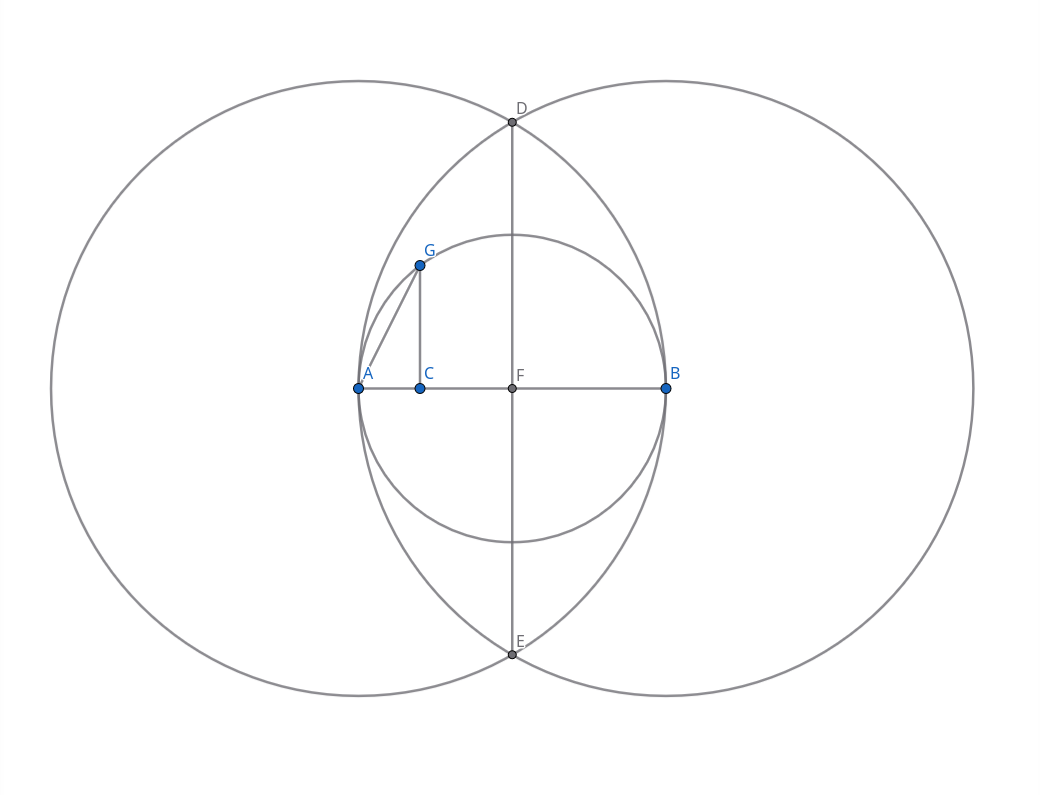
\includegraphics[scale=0.2]{fig5.png}
            \end{center}
		
	\end{enumerate}


\noindent \underline{\hspace{3in}}\\

\end{document}

